\newcommand{\ScoringLocalMax}{20.519}
\newcommand{\ScoringRestartMax}{6\,857.931}
\newcommand{\ScoringSpeedupMax}{334.23}
\newcommand{\BoundaryTraceMax}{4\,215}
\newcommand{\BoundaryReplaySpeedupMax}{14.16}
\newcommand{\BoundaryCombinedSpeedupMax}{10.31}
\newcommand{\BoundaryMomentBytes}{344\,445}
\newcommand{\BoundaryBasisBytes}{507\,862}

\newcommand{\FullTestCount}{1\,289}


\subsection{Environment, baselines, and units}

The experiments use CPython 3.12.14 on Linux x86-64. Independent native
comparisons use the Regina Python distribution 7.4.1, whose engine reports
version 7.4 \cite{Regina}. The archive contains the source inputs,
certificate-bearing records, benchmark drivers, and an environment record.
All times in the tables are wall-clock milliseconds on the research
machine; they are measurements of the stated workloads, not complexity
exponents fitted from a few points.

The all-candidate scoring comparison uses five trials per arm, alternating
which arm runs first. The final endpoint-encoding comparison uses three
alternating trials per arm on identical normal curves and mark lists.
Raw samples are retained for those paired comparisons. The literal curve
walk is capped at 200,000 represented vertices; omitted larger walks are
not timed or extrapolated. The initial exploratory records are retained
separately and are not substituted for the matched comparison.

The machine is shared. Controlled measurements were run with other heavy
research jobs paused, but hardware isolation and a distribution over
machines are not claimed. Median ratios are descriptive. They do not
include uncertainty estimates, and the complete recognizer may spend most
of its time in a different operation.

\subsection{Exact score checks and independent native moves}

The local audit evaluates all $5^5=3,125$ five-height assignments in
$\{-2,-1,0,1,2\}^5$. It compares the formulas with separate tetrahedron,
face, and edge range counts. The regression also scales heights by
$2^{20000}$ and confirms unchanged deterministic guard counts, while the
arithmetic integers themselves become longer. This checks the absence
of a loop over represented levels; it is not a claim that big-integer
arithmetic has constant cost.

A seeded mixed-move audit performs 120 moves: 63 upward and 57 downward.
The four starting inputs are layered solid tori with two and eight
tetrahedra, a one-crossing diagram exterior, and a trefoil exterior.
Each accepted move passes independent cocycle replay. Regina's separate
Pachner operation gives an isomorphic replacement triangulation, and its
normal-surface Euler characteristic agrees with the native cell count.
The observed edge-magnitude ratio attains two in an upward move, so the
factor-two bound cannot be uniformly improved for this max-norm.

The eight-tetrahedron obstruction and the connectivity counterexample
from Section~\ref{sec:splitting} are retained with complete construction
data and component certificates. The former finishes after six collapses
with two tetrahedra and one eight-piece compressing disc, saving 33 pieces
overall. The latter verifies the split into a disc and two spheres.
Neither fixture is mislabeled as a proof about an unrelated diagram.

\subsection{All eligible collapse scores: a matched comparison}

The benchmark begins with layered solid tori of sizes
$16,32,64,128,256$. Expanding disjoint pairs gives the sizes and eligible
collapse counts in Table~\ref{tab:scoring}. These triangulations have one
global vertex. Therefore two primitive cocycles for the rank-one group
differ only by overall sign: there are no nonzero vertex coboundaries.
The coherent normal vector is unchanged by that sign. This makes fresh
cohomology extraction and direct transport comparable on exactly the same
geometric outputs.

The reference arm first recognizes eligible sites without scoring them.
For every site it constructs the full replacement triangulation, extracts
a fresh primitive rank-one cocycle, and computes its Euler characteristic
and normal-disc count. The new arm obtains every score directly from the
input cochain in one scan. The driver requires equality of all per-site
Euler and piece outputs before collecting timings.

\begin{table}[htbp]
\centering
\small
\begin{tabular}{rrrrrr}
\toprule
$t$ & Sites & Bits & Local (ms) & Fresh $H^1$ (ms) & Ratio\\
\midrule
24 & 8 & 13 & 0.933 & 18.597 & 19.93$\times$\\
48 & 16 & 24 & 1.894 & 71.151 & 37.57$\times$\\
96 & 32 & 46 & 3.855 & 300.348 & 77.92$\times$\\
192 & 64 & 90 & 8.259 & 1\,300.017 & 157.40$\times$\\
384 & 128 & 179 & 20.519 & 6\,857.931 & 334.23$\times$\\
\bottomrule
\end{tabular}

\caption{Scoring all eligible collapses. Times include each arm's stated
preparation and discovery work. The speedup is the ratio of median times.
Height bits grow with the layered family.}
\label{tab:scoring}
\end{table}

At the largest measured input, direct scoring takes
\ScoringLocalMax{} ms versus \ScoringRestartMax{} ms for the fresh-extraction
arm, a \ScoringSpeedupMax{}-fold ratio. This is not a
\ScoringSpeedupMax{}-fold speedup of unknot recognition.

The comparison also has an asymptotic explanation independent of the
timings. There are $\Theta(t)$ candidate sites in this family. The reference
arm explicitly materializes a whole $\Theta(t)$-size triangulation for
each site, so those writes alone cost $\Omega(t^2)$ indexed operations.
The new scoring stage uses $O(t)$ integer operations after preparation.
Cohomology elimination, integer-bit costs, and final successful-certificate
construction are additional costs with their own bounds.

\subsection{Diagram corpus: unchanged coverage is a result}

The maintained source audit supplies 84 source cases. The experiment
selects the 82 with at most sixteen crossings, reconstructs each diagram's
canonical compact exterior, and compares three supplied-coherent-vector
strategies:
\begin{enumerate}
\item the first eligible collapse followed by a fresh tree-gauge cocycle;
\item the first eligible collapse with the original cochain transported;
\item the maximum Euler-gain, then maximum piece-saving collapse with
the original cochain transported.
\end{enumerate}
The shared descent-and-query allowance is two million cooperative guard
calls per arm, with a terminal orbit limit of 5,000 cycles. The initial
canonical exterior and seed construction precede this measured arm budget.
The separate source API charges its own full pipeline to a shared budget.

All 246 arm runs complete. Every arm performs 144 collapses in total and
finds 15 positive disc-component cases. All 30 positive transport runs
pass the independent diagram/exterior/transport/component consumer.
Thus this experiment shows no additional recognition coverage.

Final Euler characteristics agree across all three arms on all 82 sources.
The two transport policies also have identical final piece counts on every
source. Fresh gauge extraction changes that count on twelve sources:
its total is 16,170, compared with 16,297 in either transport arm.
Accordingly, these data do not establish that the score ordering produces
better final geometry than first-site transport on the ordinary diagram
corpus. They demonstrate correct reuse and identify a workload where the
proposed priority is neutral.

The corpus record contains timings for diagnosis, but they are not a
matched speed comparison. In particular, full source replay was included
for positive transport runs, and the exploratory collection briefly
overlapped another audit. The scoring table above is the controlled
performance evidence. Positive proofs are replayed again from the
packaged records; source cases whose coherent query fails remain
inconclusive rather than being classified as knotted.

\subsection{Marked-order correctness and endpoint-encoding performance}

The marked-order feature tests compare 500 seeded signed interval-exchange
multigraphs with a literal edge-occurrence oracle. One hundred further
cases compare both weight encodings on the same input. Tests include
one-vertex loops, reflection fixed points, parallel rows, adjacent marks,
singleton residual paths, empty and all-marked graphs, and directed
traversal starting at each port of an adversarial example.

The native tests use normal meridians in layered solid tori, boundary
caps, and compatible disc/sphere/M\"obius mixtures. Eighteen boundary counts
are independently compared with Regina. Source pairing order, occurrence
order, encoded integer fields, weights, claimed cycle orders, and trace
events are mutated in rejection tests. Work limits and delayed callback
exceptions are also exercised.

For the paired encoding comparison, the input is a 64-tetrahedron native
normal boundary with 89,891,140,425,706 represented vertices and four raw
interval pairings. Only the number of explicit marks changes. The moment
and one-hot arms receive the same ordered rows and marks and must return
the same solution.

\begin{table}[htbp]
\centering
\small
\begin{tabular}{rrrrrr}
\toprule
Marks & \multicolumn{2}{c}{Producer (ms)} & \multicolumn{2}{c}{Replay (ms)} & Replay\\
 & Moments & One-hot & Moments & One-hot & ratio\\
\midrule
8 & 6.482 & 7.693 & 9.987 & 15.086 & 1.51$\times$\\
32 & 32.110 & 51.145 & 72.514 & 260.093 & 3.59$\times$\\
128 & 462.465 & 710.939 & 1\,062.141 & 15\,035.489 & 14.16$\times$\\
\bottomrule
\end{tabular}

\caption{Matched endpoint encodings on one native boundary. Producer times
include certificate recording. Replay is measured separately with the
independent consumer. All times are milliseconds.}
\label{tab:encoding}
\end{table}

At 128 marks the weight dimension falls from 257 to four, while both
encodings use \BoundaryTraceMax{} AHT events. Independent replay improves
by a factor of \BoundaryReplaySpeedupMax{} in this experiment.
The serialized certificate sizes are \BoundaryMomentBytes{} bytes and
\BoundaryBasisBytes{} bytes, respectively. The retained orbit trace limits
the overall size reduction even after dense endpoint vectors are removed.

There is still substantial growth with the number of marks. The output
itself has $2p$ ports, deletion creates more interval pieces, and the orbit
trace can become longer. The four-coordinate theorem removes a growing
dimension; it does not remove all dependence on $p$ or establish a
uniform constant-factor advantage.

\begin{figure}[htbp]
\centering
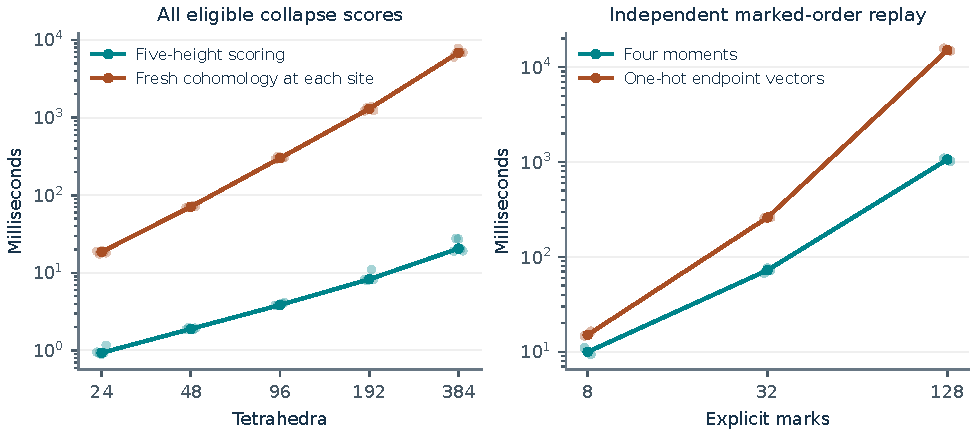
\includegraphics[width=\textwidth]{figures/paired_performance.pdf}
\caption{Paired measurements on logarithmic axes. Left: all-candidate
scoring; right: independent marked-order replay. Dots show individual
retained samples and lines join medians. No asymptotic slope is fitted.
Both comparisons require identical mathematical outputs.}
\label{fig:performance}
\end{figure}

\subsection{Literal controls and a 20,019-bit boundary size}

The retained native-boundary experiment with 22 tetrahedra, eight marks,
and 150,050 represented vertices takes 2.197 ms for the certified producer
and 3.121 ms for independent replay. The geometry-and-order wrapper takes
3.007 ms; this wrapper timing does not include the additional independent
replay. A literal native-arc walk takes 149.076 ms. Its ratio is
67.85 against the producer alone, or 28.03 against producer plus replay.
These particular medians were collected before the final callback-only
verifier correction; the interval algorithm and represented inputs are
unchanged. The final paired encoding table was regenerated after that
correction.

Small inputs favor literal walking. At 26 vertices the literal walk takes
0.046 ms versus 0.825 ms for the producer; at 1,220 vertices the times
are 1.058 ms and 1.495 ms. In 101 interleaved zero-mark controls on the
26-vertex case, moment replay takes 0.07024 ms versus 0.06827 ms for
one-hot replay, about 2.9\% slower. With one mark the corresponding
times are 0.09115 ms and 0.09023 ms. For zero or one mark the reference
dimension is one or three, so the four-coordinate representation should
not be expected to win universally.

A different input multiplies the 24-tetrahedron normal vector by
$2^{20000}$. The boundary size is
\[
 N=392836\cdot2^{20000},
\]
requiring 20,019 bits. Eight marks leave eight residual pairings from
four source rows. The recorded producer time is 8.614 ms, independent
replay 12.421 ms, and native-wrapper time 10.158 ms. The certificate
has 755,802 bytes and 108 AHT events. Three boundary components contain
marks; the remaining untouched family is retained with exact
multiplicities, giving $2^{20000}$ components overall.

This last experiment tests dependence on binary encoding and preservation
of multiplicity. It neither expands nor literally checks every represented
component, and it is not a benchmark of recognizing a knot with
$2^{20000}$ crossings.

\subsection{Regression and retained-proof validation}

The packaged snapshot passes \FullTestCount{} tests in the full
\code{unittest} discovery run, including the existing repository suite
and the new features. The retained-proof validation checks the
source-bound transport positives, the obstruction transcript, the
connectivity counterexample, and the correspondence between computed
table entries and their stored data. The machine-readable validation
record distinguishes full-suite tests, feature tests, proof replays, and
benchmark comparisons.

An initial full-suite attempt exposed a missing historical test oracle in
the standalone snapshot, not a mathematical failure. The exact pinned
\path{reports/24/reference/graded_transfer_v1.py} and the other required
historical oracle files are now included. The final full-suite run is
performed from the deliverable snapshot, with no references to an
unshipped checkout.

The validation supports this source revision and these contracts. It is
not a proof that all possible triangulations or all possible cancellation
schedules have been tested. Mathematical claims rest on the stated
proofs and hypotheses; implementation confidence additionally rests on
independent replay, adversarial examples, and the retained regression.
